\documentclass[12pt]{extarticle}
\usepackage[utf8]{inputenc}
\usepackage{cite}
\usepackage{minted}
\usepackage{hyperref}
\usepackage{graphicx,changepage}

\title{Multi-GPU training (NCCL.jl and Flux.jl)}
\author{Ziyi Xi\\
Mentors: Valentin Churavy and Tim Besard}
\date{March 2020}

\begin{document}

\maketitle

\section{Motivation}
The easiest way to speed up the training for a neural network is using GPU. However, as the models
are getting more and more complicated, using one GPU may not be sufficient. Therefore, supporting the multiple
GPU training is important. At the moment, Flux.jl only supports training on a single GPU. With the help of 
NCCL (NCCL.jl), we can distribute mini-batches into different GPUs and collect the gradient after finishing calculation
in all of the GPUs. In this proposal I'd like to talk about how I want to implement it. 

\section{What should to be implemented}

There is a package named NCCL.jl, which provides the wrapper for Nvidia's NCCL. NCCL has similar APIs comparing with 
MPI, which provides efficient communications between different GPUs, thus we don't have to look inside the low level detail of
how they are communicating with each other.

In order to use GPU to train a Flux model, we have to convert all the values to CuArray. Generally speaking, CuArray will 
work on a single GPU.  By specifying devices for different CuArrays, we can do calculation in different GPUs. However, it lacks
the ability to communicate between different devices.

By combining NCCL.jl and CuArray.jl, it's reasonable we can train a model on different GPUs, but writing everything by hand seems to 
be kind of tedious. So it's necessary to provide some APIs in Flux.jl to support divide the data into different GPUs, train the model
separately on different GPUs and collect gradients from different GPUs. This is the idea of distributing training in Flux. 

\section{The prototype of APIs}

Based on the discussion above, we should have some functions to split our dataset.
\begin{minted}[breaklines,escapeinside=||,mathescape=true, linenos, numbersep=3pt, gobble=2, frame=lines, fontsize=\small, framesep=2mm]{julia}
    split_dataset!(dataset,dataset_each_gpu)
\end{minted}

Here the dataset is the loaded data from DataLoader in Flux, and we can split the mini-batches into different GPUs. The dataset\_each\_gpu will be the splitted dataset. 

It's also essential to copy all the parameters to different devices. 
\begin{minted}[breaklines,escapeinside=||,mathescape=true, linenos, numbersep=3pt, gobble=2, frame=lines, fontsize=\small, framesep=2mm]{julia}
    copy_params!(params_in_root,params_each_gpu)
\end{minted}

During the forwarding and back propagating calculation, the code will be the same as using only a single GPU to train the model. In each GPU, 
it will calculate the averaged gradients for the weights based on all the mini-batches distributed to it. And we can call a function
to collect all the gradients and calculate the mean gradient.
\begin{minted}[breaklines,escapeinside=||,mathescape=true, linenos, numbersep=3pt, gobble=2, frame=lines, fontsize=\small, framesep=2mm]{julia}
    # assume we have already calculated the mean gradients for each GPU, gradients_this_gpu
    mean_gradients=collect_gradients(gradients_each_gpu,:mean,root=0)
\end{minted}

And based on the mean\_gradients, we can update our model. After updating the model, we can distribute the weights to all the GPUs.
\begin{minted}[breaklines,escapeinside=||,mathescape=true, linenos, numbersep=3pt, gobble=2, frame=lines, fontsize=\small, framesep=2mm]{julia}
    copy_params!(params_in_root,params_each_gpu)
\end{minted}

And do it again, we now train the model on multiple GPUs.

\section{Ways to implement the prototypes}

To implement split\_dataset!, we can use the following function in NCCL.jl:
\begin{minted}[breaklines,escapeinside=||,mathescape=true, linenos, numbersep=3pt, gobble=2, frame=lines, fontsize=\small, framesep=2mm]{julia}
    ReduceScatter!(sendbuf, recvbuf, recvcount::Integer, op, comm::Communicator; stream::CuStream=CuDefaultStream() )
\end{minted}

However, based on the meaning of ReduceScatter!, we have to provide in1, in2, in3 as illustrated in the document for NCCL.
\begin{figure}[ht]
    \centering
         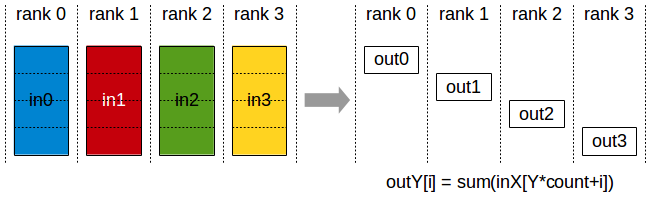
\includegraphics[width=1.0\textwidth]{reducescatter}
          \caption{ReduceScatter (from NCCL document)}
\end{figure}
The idea is that we can provide an empty in1, in2, and in3. This difficulty is from the fact that NCCL has not provided 
the point to point communication yet. (see \url{https://github.com/NVIDIA/nccl/issues/212})

To implement copy\_params!, it's simply the broadcast:
\begin{minted}[breaklines,escapeinside=||,mathescape=true, linenos, numbersep=3pt, gobble=2, frame=lines, fontsize=\small, framesep=2mm]{julia}
    Broadcast!(sendbuf, recvbuf, count::Integer, root::Int, comm::Communicator; stream::CuStream=CuDefaultStream() )
\end{minted}
\begin{figure}[ht]
    \centering
         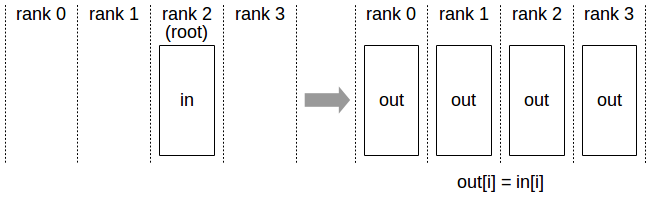
\includegraphics[width=1.0\textwidth]{broadcast}
          \caption{Broadcast (from NCCL document)}
\end{figure}


And to implement collect\_gradients, using Reduce is reasonable:
\begin{minted}[breaklines,escapeinside=||,mathescape=true, linenos, numbersep=3pt, gobble=2, frame=lines, fontsize=\small, framesep=2mm]{julia}
    Reduce!(sendbuf, recvbuf, count::Integer, op, root::Int, comm::Communicator; stream::CuStream=CuDefaultStream() )
\end{minted}
\begin{figure}[ht]
    \centering
         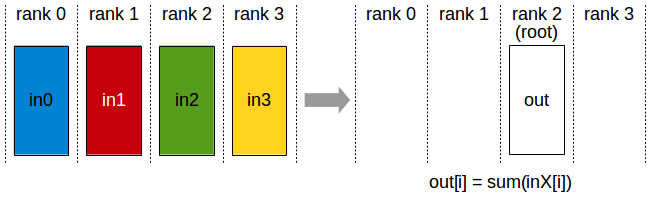
\includegraphics[width=1.0\textwidth]{reduce}
          \caption{Reduce (from NCCL document), will use mean as the operator.}
\end{figure}

\newpage
\section{Others to do with NCCL.jl and Flux.jl}

At the moment, NCCL.jl has already done an awesome job in wrapping NCCL. However, the APIs are low level wrappers at the moment.
So I am planning to firstly wrap the low level APIs into some high level APIs, for example:

In NCCL.jl/src/collective.jl, Allreduce!, we have the parameters sendbuf and recvbuf, which are actually of the type CuPtr\{Cvoid\}.
In practice, it will be nice if we can support to use the type CuArray instead. There are lots of cases like that and it should be done at the
beginning of this project.

As for Flux.jl, it's reasonable to support different kinds of using cases:
\begin{itemize}
    \item single process/thread for single GPU (use MPI)
    \item one process/thread for all GPUs 
    \item one process/thread for some GPUs (use MPI)
\end{itemize}

From the document of MPI.jl (\url{https://juliaparallel.github.io/MPI.jl/latest/usage/#CUDA-aware-MPI-support-1}), it supports CUDA-aware MPI, which is a great feature to be implemented here.


\section{Project Timeline}
\begin{itemize}
    \item{\textbf{before starting}} Talk with advisors to set goals for each week, and get me more familiar with NCCL and CuArray.
    \item{\textbf{week 1}} Help develop the high level wrapper for NCCL.jl.
    \item{\textbf{week 2}} Write test and do benchmarks for NCCL.jl.
    \item{\textbf{week 3-4}} Develop the prototype functions.
    \item{\textbf{week 5}} Write test and do benchmarks for the written code.
    \item{\textbf{week 6}} Implement the distributing training for some models in the model zoo, and do benchmark.
    \item{\textbf{week 7-8}} Write high level wrappers for distributing training code, and make pull requests to the master branch of Flux.jl.
    \item{\textbf{week 9-11}} Buffer time to solve problems, prettify the code, and do things that has not been considered in this proposal.
\end{itemize}

\section{About me}
I am currently a Ph.D student in the department of computational mathematics, science and engineering from Michigan State University. And my main 
research focus is on computational seismology. I get my bachelor degrees in computer science and geophysics from the University of Science and Technology of
China.

I am familiar with coding in Julia, Python, C++, Fortran, CUDA and Javascript. Since I am studying and working on the computational science, 
I am more fond of techniques on high performance computing and heterogeneous computing.

My github user name is ziyixi, and there are some packages I have developed to help with my research. One example is seisflow, which is a python package 
to help with doing full seismic waveform inversion in seismology to invert for the velocity structure of Earth. Into this package, I am also using
Julia to process my result \url{https://github.com/ziyixi/seisflow/tree/master/seisflow/julia/specfem_gll.jl/src/program}. 

I have some experience in using CUDA from C++ several years ago in my undergraduate, and it's really efficient though hard to write the code. Luckily we have 
CuArray.jl, and it's much more easier to write the code now. I have also took some classes in deep learning and familiar with using Pytorch, which may 
be a good help for me to do this project.

My email address is xiziyi@msu.edu and my personal website is \url{https://ziyixi.github.io/} which may still be in development. I would appreciate it if I 
could be selected to the program this year, and contribute to the Julia community.

\end{document}